% this is a comment -- it is a line starting in %

% the pre-eamble is everything from \documentclass to \begin{document}
\documentclass[12pt]{article} % the 12pt makes the font bigger
\title{Math 480: Lectures 11 -- Latex (2 of 3)}  % document title
\author{William Stein}   % who wrote this
\date{April 20, 2016}

\usepackage{amssymb}

\usepackage{hyperref}  % make it so there is a \url{} command and links work (in pdf!)

% include support for putting pdf's and png's in our file
\usepackage{graphicx}

% Package for the "newtheorem" command
\usepackage{amsthm}
\newtheorem{exercise}{Exercise}[section]   % exercise environment

\begin{document}
% this is the body of the document

% This is a command that says: "put the title block here".
% Try copying this command and putting it somewhere else and get multiple titles
\maketitle

\tableofcontents

% Use \section{...} to make a new section.
\section*{Reminders\label{reminders}}

{\bf Some reminders:}  % md the {\bf ...} makes it bold

\begin{enumerate}
\item Start screencast!
\item You should open {\tt lectures/2016-04-20/2016-04-20.tex} in your project
\item \label{reminder-homework} Homework and peer grading due Friday at 6pm. (Questions?)
\end{enumerate}

\section{Math formulas}
\LaTeX is massively different than Microsoft Word.  You focus
entirely on the content and structure of what you are
writing, not on how it looks.  Also, the result is much more
professional looking.   And you can define functions, e.g.,

\newcommand{\hello}[1]{Hello #1, hello #1 !! }

\hello{World} - I say \hello{to you}!

\subsection{Some basics}
Google ``latex symbols''\footnote{Look in the tex file for how I did those quotes and this footnote.} for tables giving how to typeset
interesting symbols, like this:
$$
\varphi, \Xi, \partial, \hookleftarrow, \bigoplus
$$

Consider $\varphi + \Xi^3$.

Top hit (and I'm having dinner with them on Friday):\\ \url{https://www.artofproblemsolving.com/wiki/index.php/LaTeX:Symbols}

This webpage explains a lot of math typesetting.  Here's
some key things:
\begin{itemize}
\item Braces: $\{ x : x \in \mathbb{Q}\}$
\item Powers: $x^{2+3}$,    $x^2+3$,  $x^(2+3)$
\item Subscripts: $x_2, x_5, x_{2+3}$
\item Both: $x^{2+3}_{5}$
\item A fraction: $\frac{2+3 \hello{10}}{5}$
\item An integral: $\int_0^{\pi+e^i} \sin(x) dx$
\item A ``displayed'' integral: $$\int_0^{\pi} \sin(x) dx$$
\end{itemize}

\url{http://detexify.kirelabs.org/classify.html}

\subsection{Using Sage}

Given any object {\tt obj} in a Sage worksheet you
can (try to) do {\tt latex(obj)} to see how to typeset
obj.   You already learned about sagetex, which uses
this under the hood, on Monday.

$$
x + \frac{1}{6} x^{3} + {(-\frac{1}{40})} x^{5} + {(-\frac{55}{1008})} x^{7} + \mathcal{O}\left(x^{8}\right)
$$

$$
\displaystyle \left(\begin{array}{rrr}
1 & -2 & \frac{1}{2} \\
1 & 0 & 0 \\
-2 & 0 & 1
\end{array}\right)
$$

\begin{exercise}
Use Sage to find a latex formula for the first few terms
of the Taylor series of $\tan(x)$ about
zero.\footnote{Hint: use {\tt latex(tan(x).series(x, 10))} in a worksheet, then copy/paste.}
\end{exercise}

$$
your series here!
$$


\begin{exercise}
Use Sage to Find a latex formula for a matrix using Sage.  Use the command {\tt matrix} to make a matrix.
\end{exercise}

$$
your matrix here!
$$




\subsection{Use Some random webpage}

If you do a Google search for {\tt latex formula editor}
you'll find (many) kind-of-ugly websites with
various programs that
let you graphically construct an equation, which show
you the latex code.

This is an unusual new demo, where they use machine learning
to recognize handwriting (it is pretty impressive):\\
\url{http://webdemo.myscript.com/#/demo/equation}

$$
\frac{\Omega +\alpha ^{3}} {2}
$$

\section{Sectioning and cross referencing\label{a-label}}
This is Section \ref{a-label}.  The next section is Section \ref{graphics}.
You can reference anything, e.g., reminder \ref{reminder-homework}
from Section \ref{reminders}.

\begin{exercise}
Try reordering the enumerate list above in some random way and or the sections
(or adding new ones), then recompile and see all the cross reference numbers
get updated.
\end{exercise}


\section{Including graphics\label{graphics}}

You can take any pdf, png, or jpg file, put it in the
same directory as your tex file (+New, drag and drop),
and display them as follows:

\begin{center}  % this centers it
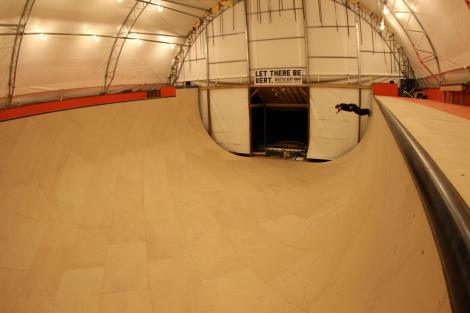
\includegraphics[width=.6\textwidth]{svr.jpg}
\end{center}

\hello{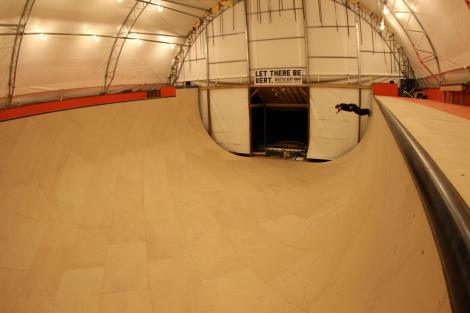
\includegraphics[width=.1\textwidth]{svr.jpg}}

$$x^{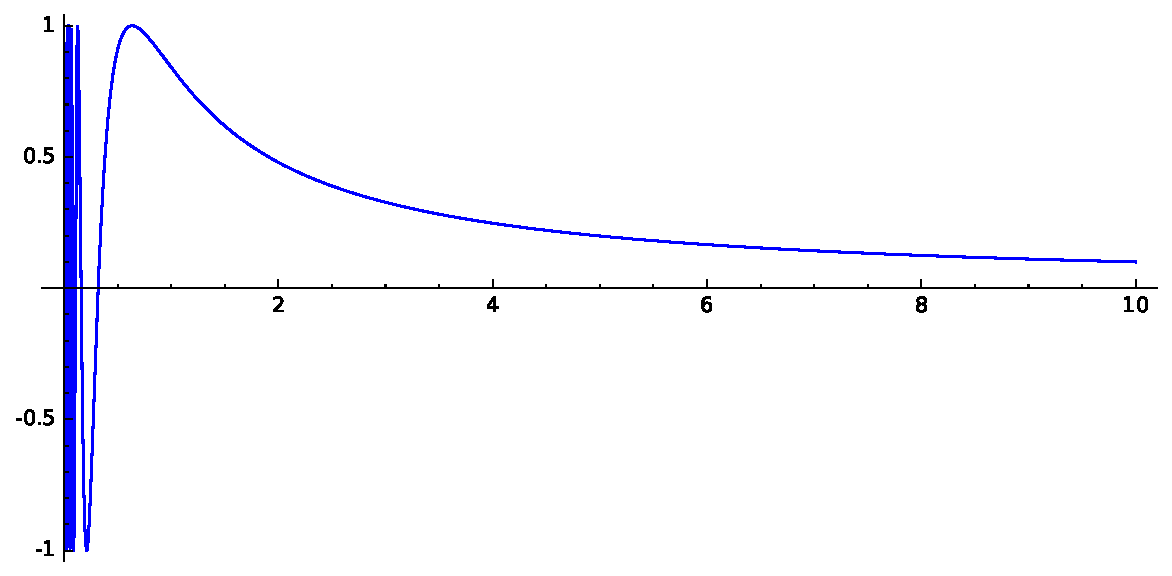
\includegraphics[width=.1\textwidth]{a.pdf}} + 1$$

\begin{exercise}
Upload and insert an image of your choice below.  It must
be png or pdf.
\end{exercise}

% Copy paste the includegraphics thing above here, change
% the name from image to the name of your file:



Sage can also produce pdf's of plots.
E.g., if {\tt g = plot(sin) + plot(cos)}, then
{\tt g.save('a.pdf')} will create a file {\tt a.pdf}
that you can include.  This is a little more tedious
than Sagetex, but you have more control.

\begin{exercise}
Create a plot and save it to a file
as above in a Sage worksheet, then include it below:
\end{exercise}

% Copy paste the includegraphics thing above here, change
% the name from image to the name of your file:




\end{document}
